\documentclass[german=false,thesistype=master,nolistoftables,noabstract]{tubsthesis}

\usepackage{lipsum}
\usepackage{pdfpages}								% Einbinden von PDF-Pages

\thesisname{Johanna Doe}
\thesismatrikel{1234567}
\thesisemail{j.doe@tu-braunschweig.de}
\thesismajor{Informatik}
\thesisduration{3}
\thesissupervisors{Super Visor, M. Sc.}{Dr. Dipper Visor}{}
\thesisprofessor[Prof.\,Dr.-Ing.\,Jane Smith]{Prof.\,Dr.-Ing.\,Lars Eisbär}
\thesistitle{Titel der Thesis}{Title of the thesis}
\thesisbegindate{2020-01-01}
%\thesisenddate{2020-01-02}
\thesispresentationpoints{5.7}

\addbibresource{bibliography.bib}

\thesisinstitute{Institute of Perfect Writing in IT}

\begin{document}
    \thesisabstract{%
        % Since `noabstract` is set, this abstract won't be printed
        This is an english text.\\
        \lipsum[1-2]
    }
    
    \begin{thesis}

        \chapter{Introduction}

        \lipsum[1-3]

        \begin{figure}
        \centering
        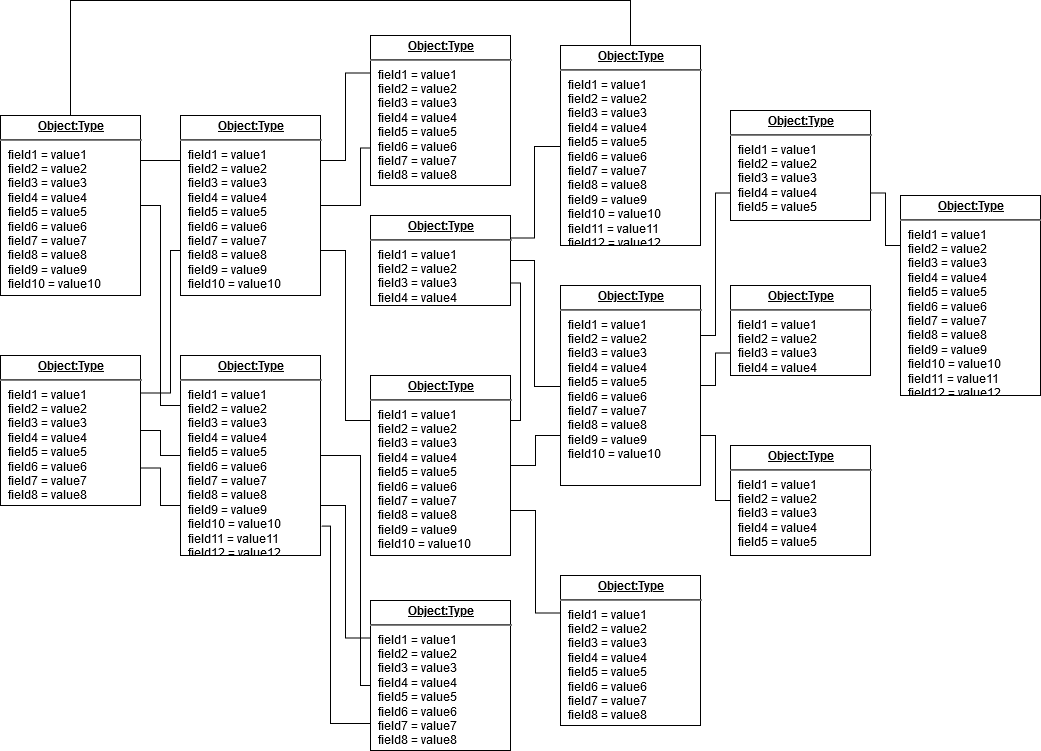
\includegraphics[width=\textwidth]{images/example_diagram.png}
        \caption{Some diagram, not relevant to anything~\cite{lisa}}
        \label{fig:inga}
        \end{figure}

        \lipsum[4-7]

    \end{thesis}

    
\includepdf[pages=-]{./Deckblatt/2099_StA_Name_Deckblatt.pdf}

\chapter*{Declaration}
Hiermit versichere ich, Lucas Hermann, durch meine Unterschrift, dass ich die
vorliegende Masterarbeit mit dem Titel ``<<Titel>>'' selbständig und ohne Benutzung
anderer als der angegebenen Hilfsmittel angefertigt habe. Alle Stellen, die wörtlich oder sinn-
gemäß aus veröffentlichten oder unveröffentlichten Schriften entnommen sind, habe ich als
solche kenntlich gemacht. Insbesondere sind auch solche Inhalte gekennzeichnet, die von
betreuenden wissenschaftlichen Mitarbeiterinnen und Mitarbeitern des Instituts für Akustik eingebracht wurden.

Die Arbeit oder Auszüge daraus haben noch nicht in gleicher oder ähnlicher Form dieser
oder einer anderen Prüfungsbehörde vorgelegen.

Mir ist bewusst, dass Verstöße gegen die Grundsätze der Selbstständigkeit als Täuschung
betrachtet und entsprechend der Prüfungsordnung geahndet werden.

\begin{flushright}
Braunschweig, \today
\end{flushright}

\vspace{2cm}
\hspace{2cm}\rule{5cm}{1pt}

\hspace{2cm}\small{Lucas Hermann} 

\chapter*{Abstract}
\lipsum[1]

\tableofcontents


\chapter{Introduction}

\textcolor{tubsSecondary}{Dies ist ein Text in \texttt{tubsSecondary}.}
\textcolor{tubsViolet}{Dies ist ein Text in \texttt{tubsViolet}.}
\textcolor{tubsGreenDark}{Dies ist ein Text in \texttt{tubsGreenDark}.}\bigskip

\lipsum[1]

\begin{itemize}
  \item Aufzählungspunkt Eins
  \item Aufzählungspunkt Zwei
    \begin{itemize}
      \item Unter-Aufzählungspunkt Eins
      \item Unter-Aufzählungspunkt Zwei
    \end{itemize}
  \item Aufzählungspunkt Drei
\end{itemize}

\chapter{Theoretical Background of statFEM}

\lipsum[2-5] %\cite{campolina}

\chapter{1D Example and Application in Vibroacoustics}

\lipsum[2-5] %\cite{campolina}



\chapter{Results and Discussion}

\lipsum[1-3] %\cite{Langer2019}

\section{Section 1}

\lipsum[4-7] %\cite{Yaghoubi:2017}

\end{document}